\documentclass{beamer}
\usepackage[pdftex]{graphicx}
\usetheme{Malmoe}
\begin{document}
  \title{Knowledge Advantage Desktop}
  \subtitle{Interface, Infrastructure, and Markup}
  \author{Larry Reaves}
  \frame{\titlepage}
  \begin{frame}
    \frametitle{Introduction}
    KAD assists in managing the vast amounts of information that is available, yet difficult to locate and parse.
    It can assist in\\
    \begin{itemize}
    \item{discovering new content}
    \item{evaluating the contents of documents}
    \item{finding relationships between documents}
    \item{visualizing how documents are connected}
    \end{itemize}
  \end{frame}
  \begin{frame}
    \frametitle{Interface}
    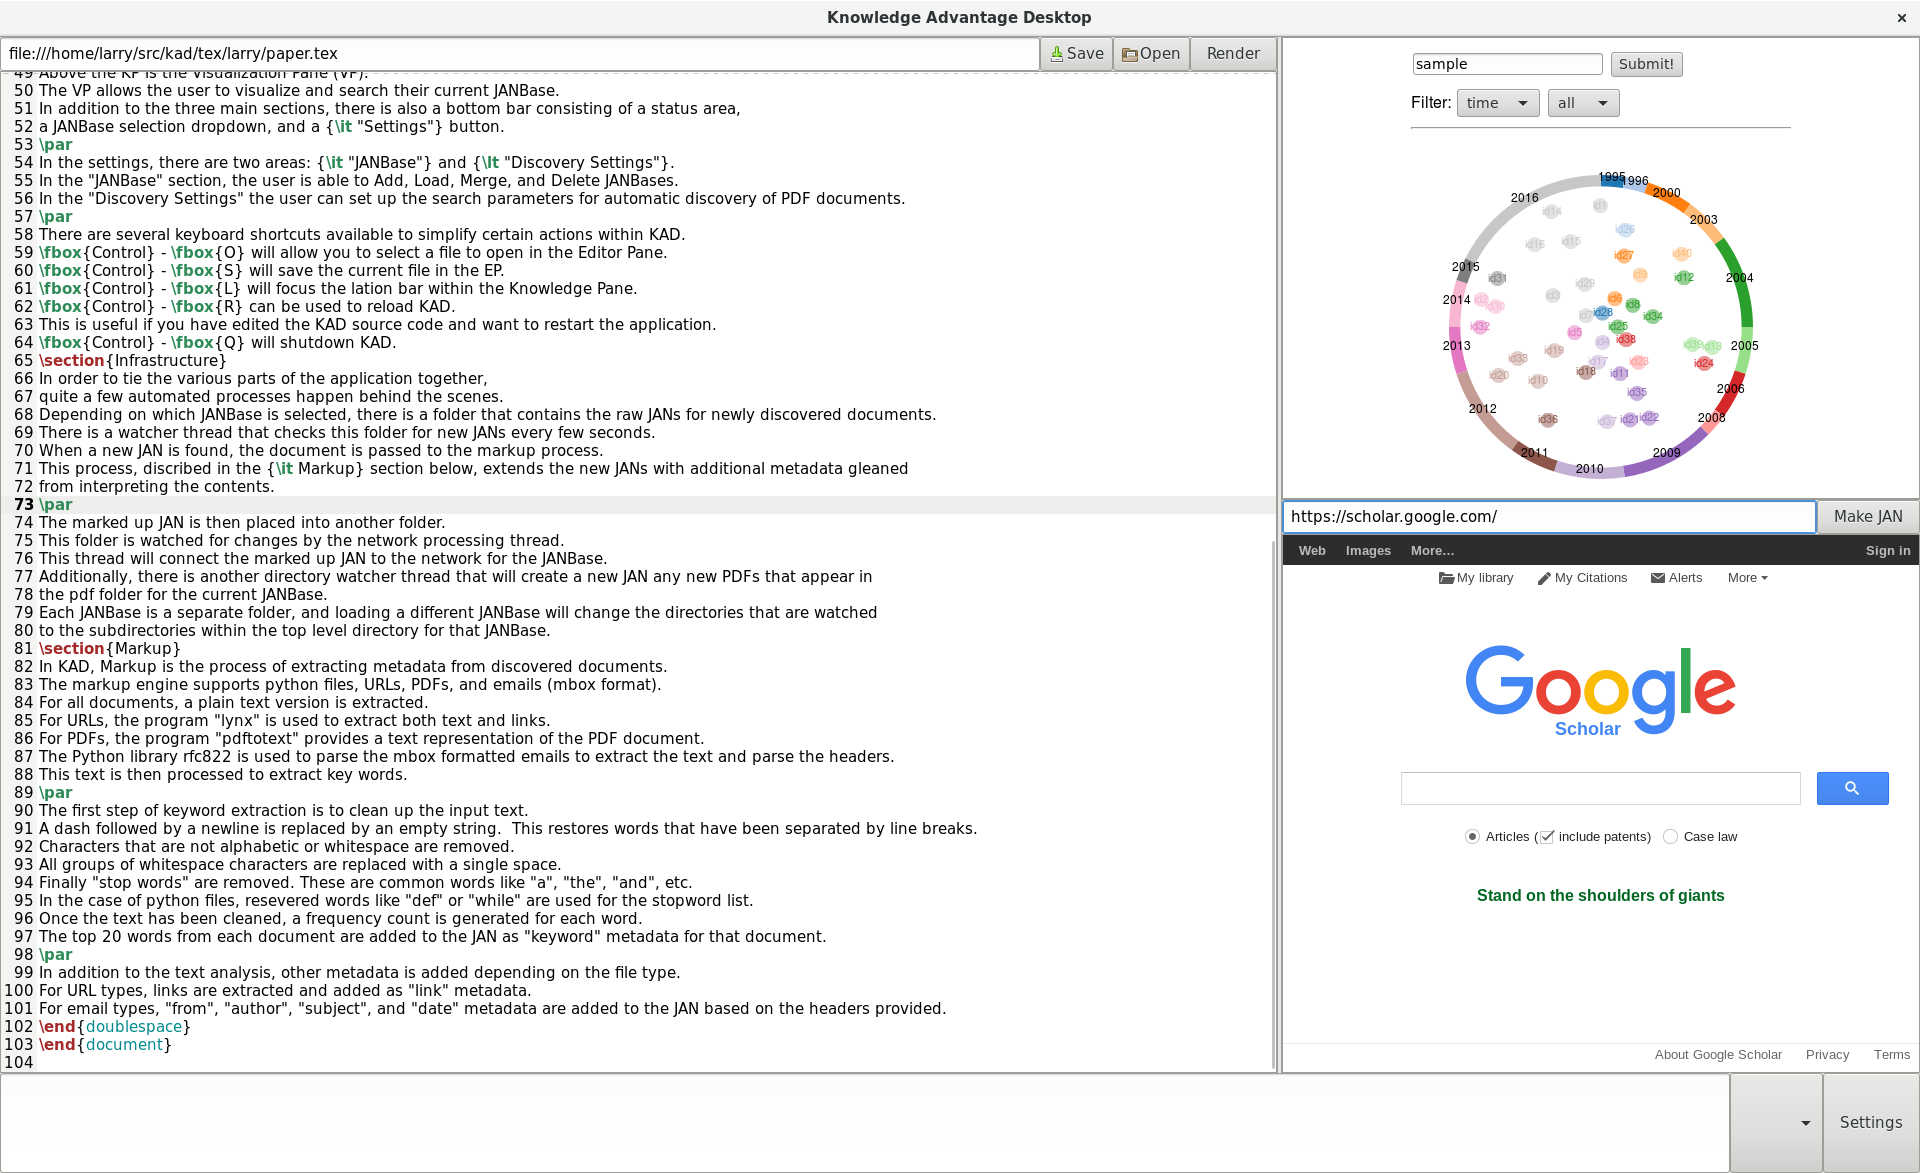
\includegraphics[width=3in]{images/kad-overview.png}\\
    The KAD interface consists of three resizable areas\\
    \begin{itemize}
    \item{Editor Pane for producing content}
    \item{Knowledge Pane for viewing URL and PDF documents}
    \item{Visualization Pane for viewing and searching the current JANBase network}
    \end{itemize}
  \end{frame}
  \begin{frame}
    \frametitle{Infrastructure}
    The KAD has several automated processes to turn discovered documents into networked JANs in the JANBase\\
    \begin{itemize}
    \item{DirWatcher threads to check for new PDFs to create JANs for}
    \item{DirWatcher threads to check for new JANs for mark up}
    \item{Email thread to download new mail and create JANs}
    \item{Networking thread to link marked up JANs into the JANBase}
    \item{Each JANBase has its own folder and all of these threads operate on the currently selected JANBase}
    \end{itemize}
  \end{frame}
  \begin{frame}
    \frametitle{Markup}
    The software automatically annotates documents\\
    \begin{itemize}
    \item{Extracts text from PDFs, URLs, text files, emails}
    \item{Performs frequency analysis to extract the top 20 words in the text}
    \item{Extracts links from HTML documents}
    \item{Extracts headers from emails}
    \end{itemize}
  \end{frame}
\end{document}